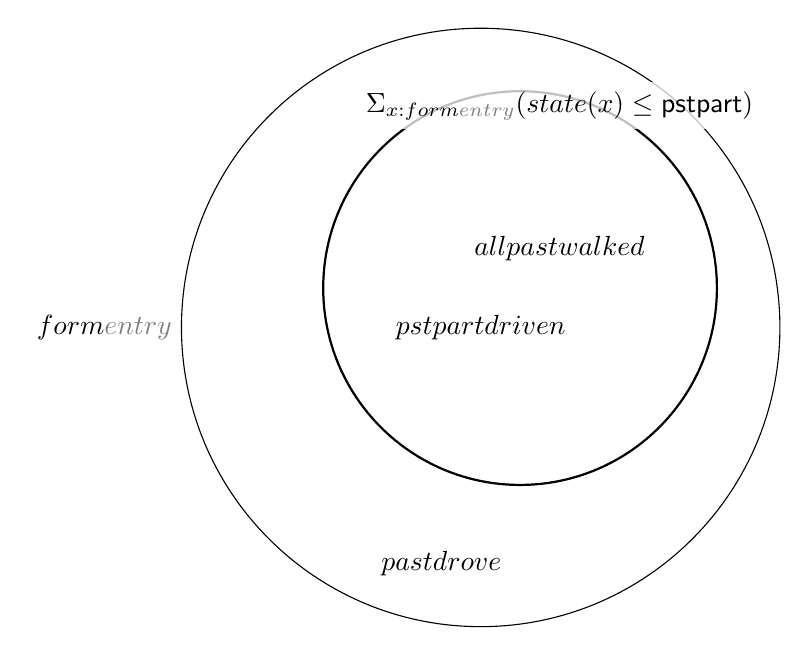
\begin{tikzpicture}
  \node (a) at (0,0) {$\sformt{\red pstpart}{driven}$};
  \node (b) at (-0.5,-3) {$\sformt{\red past}{drove}$};
  \node (c) at (1,1) {$\sformt{\red allpast}{walked}$};
  
  \draw (0,0) circle (3.8) (-3.8,0) node [left] {$form\mathcolor{gray}{entry}$};
  \draw[thick] (0.5,0.5) circle (2.5) (1,2.5) node [above,fill=white,fill opacity=0.75,text opacity=1] {$\Sigma_{x:form\mathcolor{gray}{entry}}(state(x)\leq \mathsf{pstpart})$};
\end{tikzpicture}

%%% Local Variables:
%%% mode: latex
%%% TeX-master: "../../morphology"
%%% End:
